\documentclass[supercite]{Experimental_Report}

\title{~~~~~~计算机视觉实验一~~~~~~}
\author{崔昊阳}
\school{计算机科学与技术学院}
\classnum{CS2104}
\stunum{U202115415}
\instructor{刘康}
\date{2023年12月7日}

\usepackage{algorithm, multirow}
\usepackage{algpseudocode}
\usepackage{amsmath}
\usepackage{amsthm}
\usepackage{framed}
\usepackage{mathtools}
\usepackage{subcaption}
\usepackage{xltxtra}
\usepackage{bm}
\usepackage{tikz}
\usepackage{tikzscale}
\usepackage{pgfplots}
\usepackage{listings}
\lstset{
    backgroundcolor = \color{white},    % 背景色
    basicstyle = \small\ttfamily,           % 基本样式 + 小号字体
    rulesepcolor= \color{white},             % 代码块边框颜色
    breaklines = true,                  % 代码过长则换行
    numbers = left,                     % 行号在左侧显示
    numberstyle = \small,               % 行号字体
    keywordstyle = \color{blue}\bfseries,      % 关键字颜色
	identifierstyle=\color{purple}, 		% 标识符颜色
    commentstyle =\color{green},        % 注释颜色
    stringstyle = \color{green},          % 字符串颜色
    frame = shadowbox,                  % 用(带影子效果)方框框住代码块
    showspaces = false,                 % 不显示空格
    columns = flexible,                    % 字间距固定
}

\pgfplotsset{compat=1.16}

\newcommand{\cfig}[3]{
  \begin{figure}[H]
    \centering
    \includegraphics[width=#2\textwidth]{images/#1.tikz}
    \caption{#3}
    \label{fig:#1}
  \end{figure}
}

\newcommand{\sfig}[3]{
  \begin{subfigure}[b]{#2\textwidth}
    \includegraphics[width=\textwidth]{images/#1.tikz}
    \caption{#3}
    \label{fig:#1}
  \end{subfigure}
}

\newcommand{\xfig}[3]{
  \begin{figure}[H]
    \centering
    #3
    \caption{#2}
    \label{fig:#1}
  \end{figure}
}

\newcommand{\rfig}[1]{\autoref{fig:#1}}
\newcommand{\ralg}[1]{\autoref{alg:#1}}
\newcommand{\rthm}[1]{\autoref{thm:#1}}
\newcommand{\rlem}[1]{\autoref{lem:#1}}
\newcommand{\reqn}[1]{\autoref{eqn:#1}}
\newcommand{\rtbl}[1]{\autoref{tbl:#1}}

\algnewcommand\Null{\textsc{null }}
\algnewcommand\algorithmicinput{\textbf{Input:}}
\algnewcommand\Input{\item[\algorithmicinput]}
\algnewcommand\algorithmicoutput{\textbf{Output:}}
\algnewcommand\Output{\item[\algorithmicoutput]}
\algnewcommand\algorithmicbreak{\textbf{break}}
\algnewcommand\Break{\algorithmicbreak}
\algnewcommand\algorithmiccontinue{\textbf{continue}}
\algnewcommand\Continue{\algorithmiccontinue}
\algnewcommand{\LeftCom}[1]{\State $\triangleright$ #1}

\newtheorem{thm}{定理}[section]
\newtheorem{lem}{引理}[section]

\colorlet{shadecolor}{black!15}

\theoremstyle{definition}
\newtheorem{alg}{算法}[section]

\def\thmautorefname~#1\null{定理~#1~\null}
\def\lemautorefname~#1\null{引理~#1~\null}
\def\algautorefname~#1\null{算法~#1~\null}

\begin{document}

\maketitle

\clearpage

\pagenumbering{Roman}

\tableofcontents[level=2]

\clearpage

\pagenumbering{arabic}

\section{实验要求}
任务要求:设计一个前馈神经网络,对一组数据实现分类任务。

下载 “dataset.csv” 数据集,其中包含四类二维高斯数据和它们的标签。设计至少含有一层隐藏层的前馈神经网络来预测二维高斯样本(data\_1,data\_2)所属的分类label。这个数据集需要先进行随机排序,然后选取90\%用于训练,剩下的10\%用于测试。

注意事项:
\begin{enumerate}
	\item 深度学习框架任选。
	\item 鼓励尝试不同的网络层数、不同的神经元个数、使用不同的激活函数等,观察网络性能。
	\item 实验报告需包含神经网络架构、每一轮 mini-batch 训练后的模型在训练集和测试集上的损失、最终的训练集和测试集准确率,以及对应的实验分析。
	\item 将代码和实验报告打包成 ZIP 压缩包,以 “姓名-学号-实验报告\#” 命名,比如“张三-2020XXX-实验报告一.zip”,提交到学习通。
	截止时间为12月20号下午2:00。
\end{enumerate}

\section{数据处理}
本次实验的数据由 4 类不同的二维空间中的点组成。它们来自 4 个不同的高斯分布。

首先我们进行数据探索。经过观察,我们发现,所有的数据没有缺失或异常。所有我们无需进行数据清洗。
接下来,我们统计 4 种类别的样本个数,如图\ref{数据个数分布图}所示。从图中我们可以看出,四种类别的样本个数均为 1000 个。
没有类别不平衡的现象。然后,我们作出数据分布图,如图\ref{数据分布图}所示。我们发现,四类样本均大致满足高斯分布,但是分布较为分散,
较难和其它样本完全分开。最后,我们对这四类样本满足的高斯分布进行了拟合。
拟合结果如图\ref{数据分布拟合图}所示,拟合参数的值如表\ref{拟合参数}所示。至此,数据探索完成。
\begin{figure}[H]
	\begin{center}
		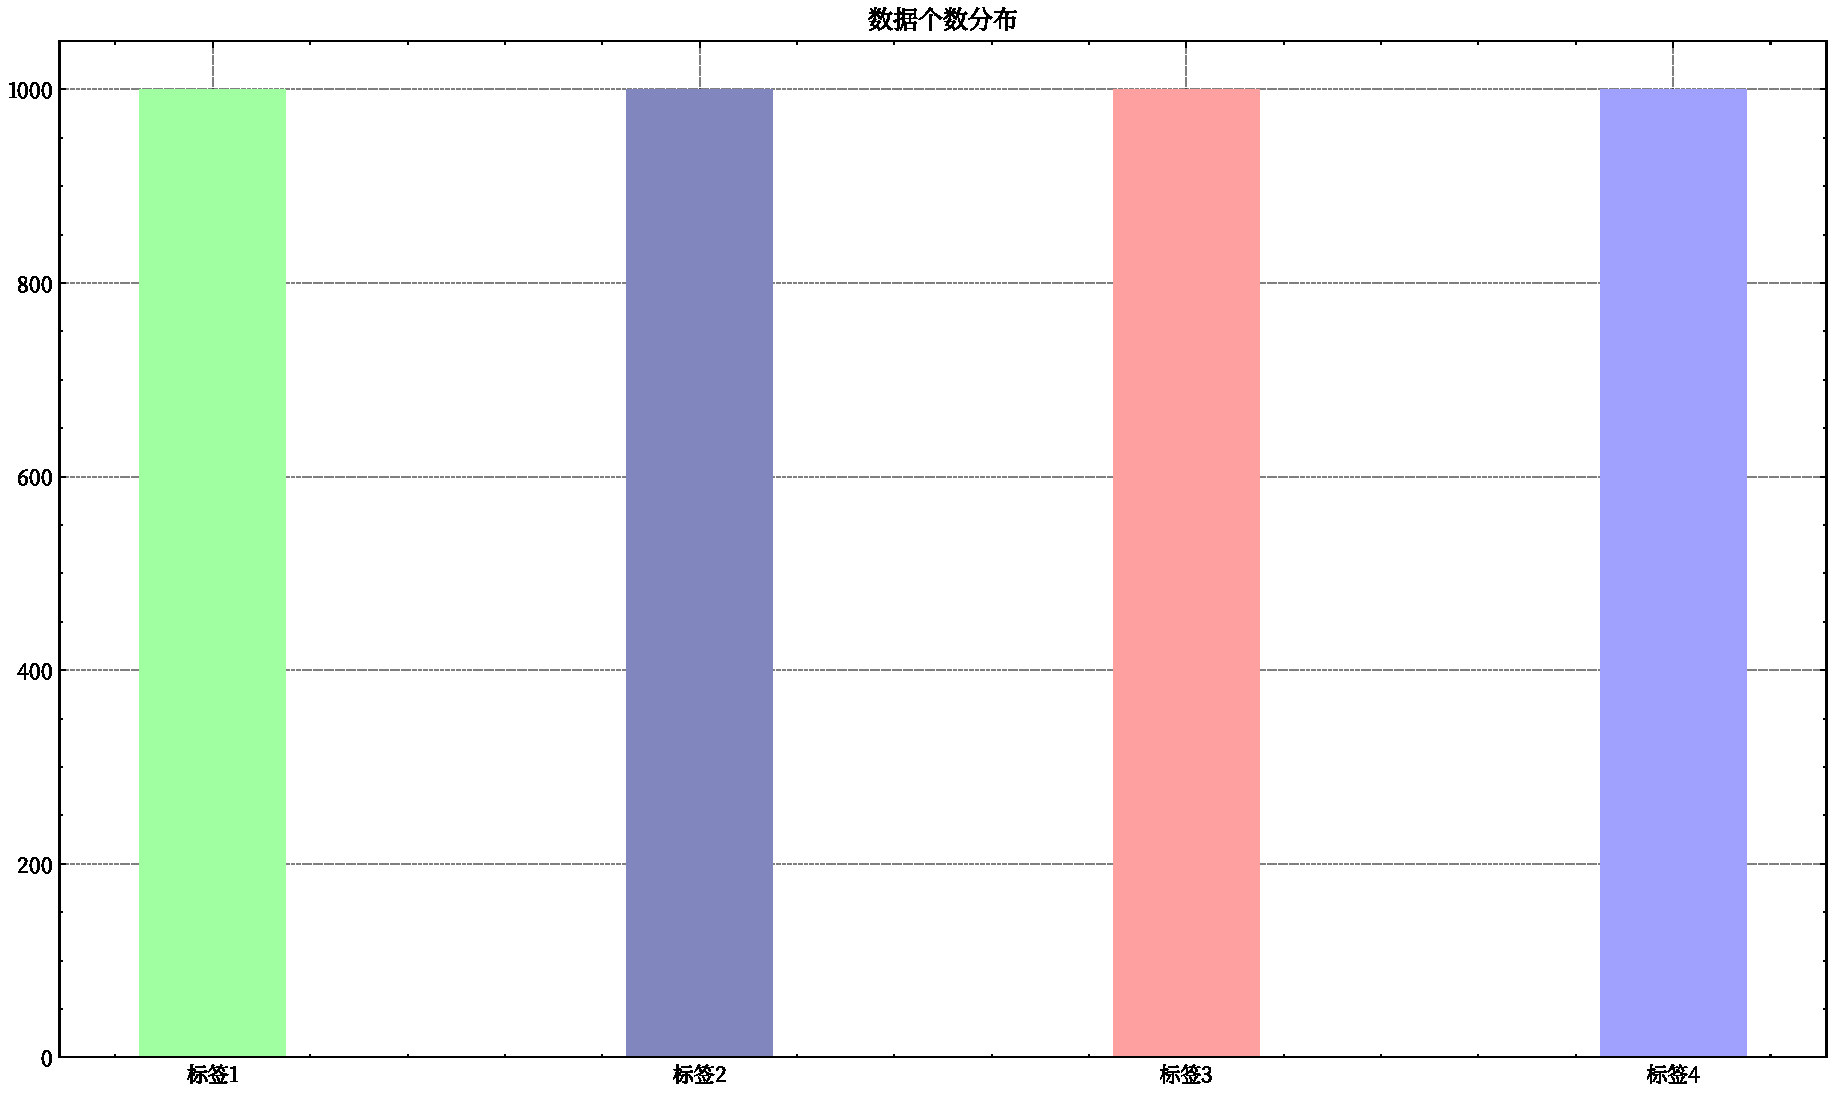
\includegraphics[scale=0.30]{../images/数据个数分布图.pdf}
		\caption{数据个数分布图}
		\label{数据个数分布图}
	\end{center}
\end{figure}
\begin{figure}[H]
	\begin{center}
		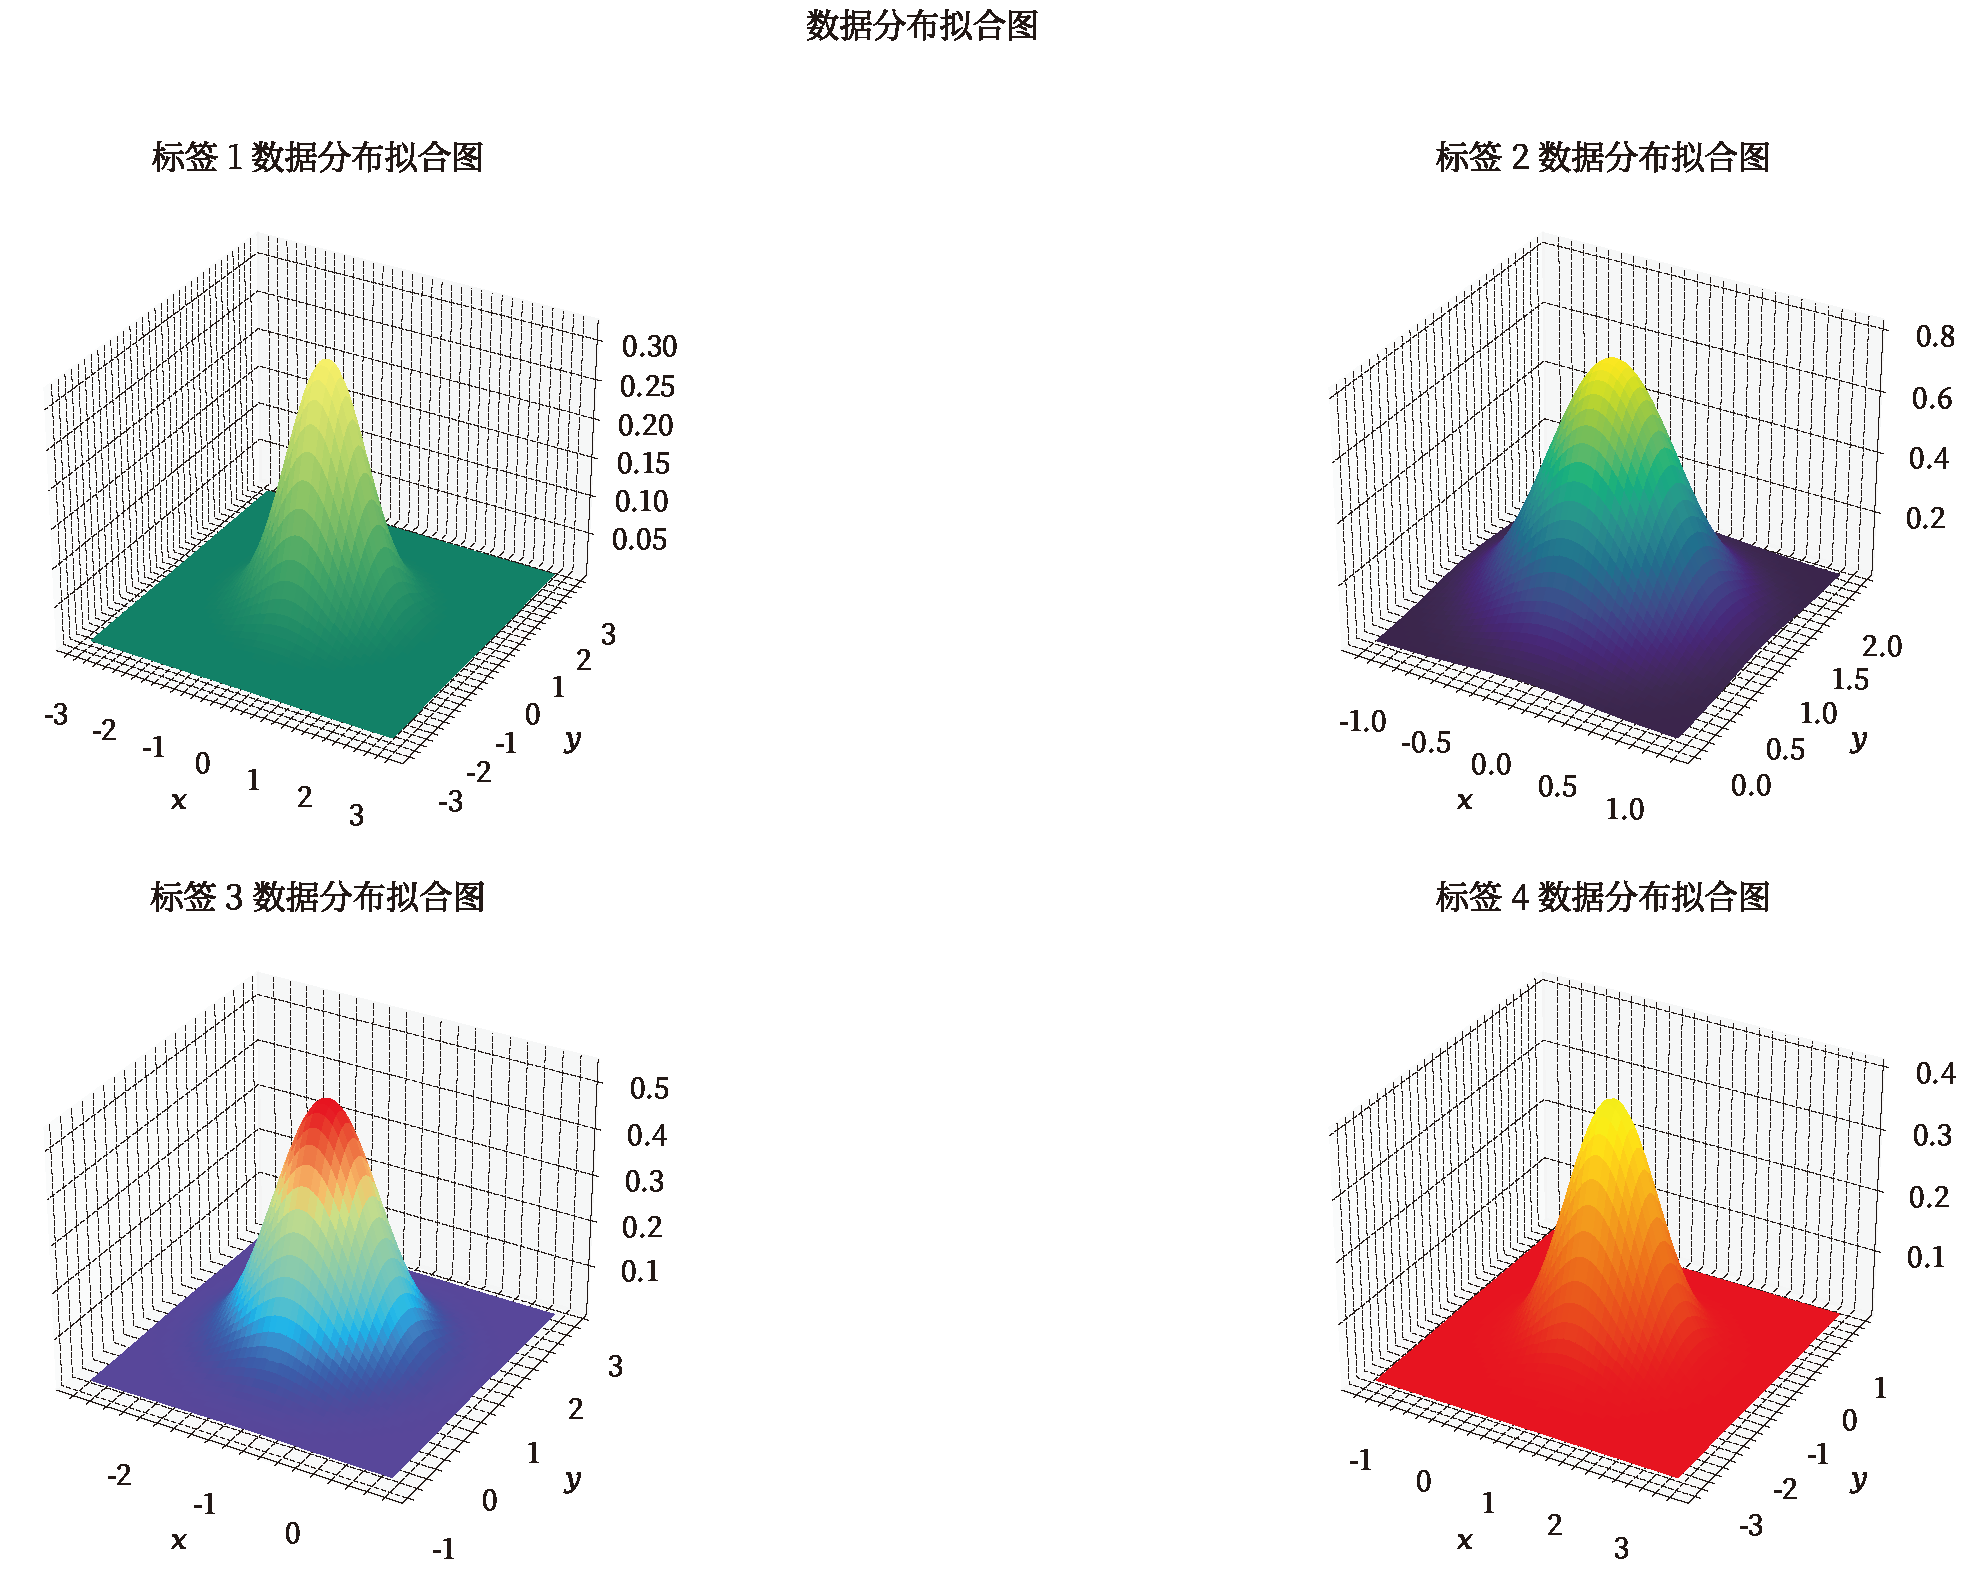
\includegraphics[scale=0.35]{../images/数据分布拟合图.png}
		\caption{数据分布拟合图}
		\label{数据分布拟合图}
	\end{center}
\end{figure}
\begin{figure}[H]
	\begin{center}
		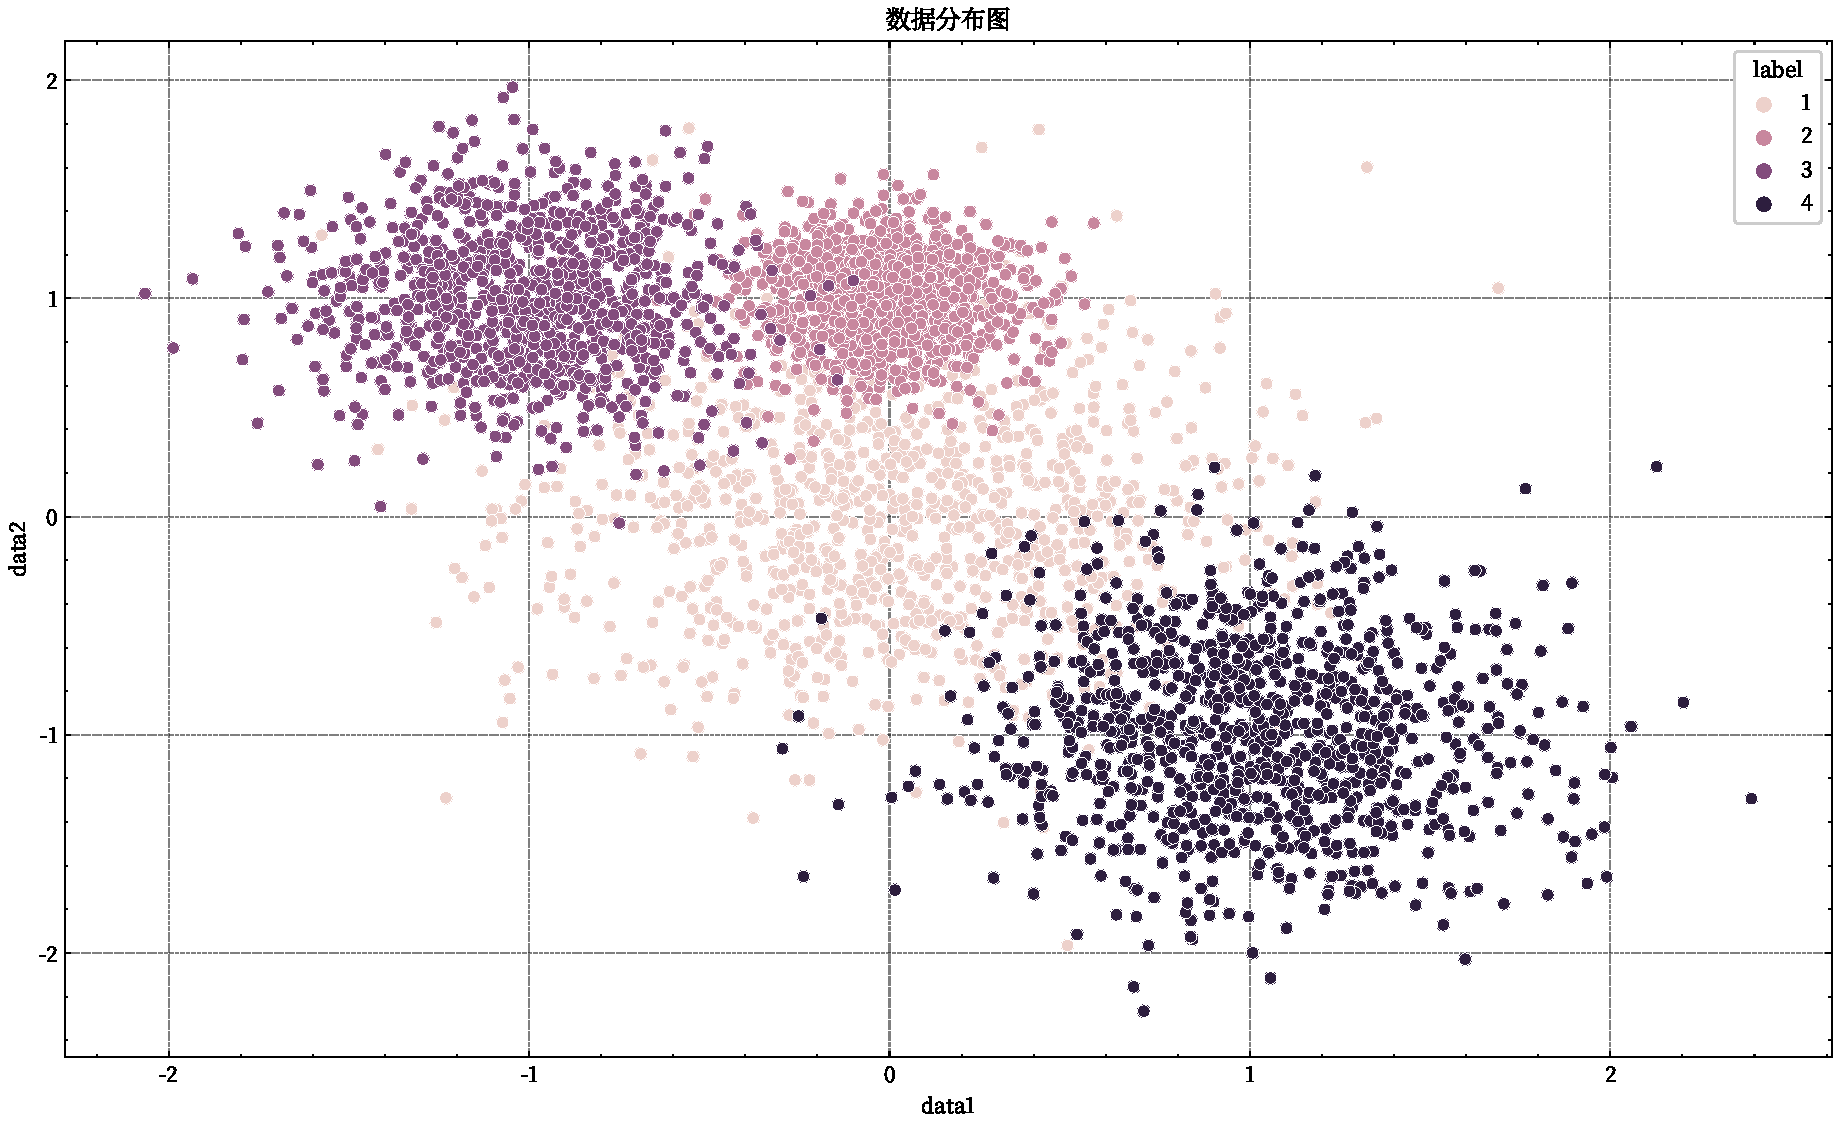
\includegraphics[scale=0.40]{../images/数据分布图.pdf}
		\caption{数据分布图}
		\label{数据分布图}
	\end{center}
\end{figure}
\begin{table}[H]
	\centering
	\caption{拟合参数表}
	  \begin{tabular}{ccccc}
		\toprule
	  \textbf{label} & \textbf{data1 均值} & \textbf{data1 标准差} & \textbf{data2 均值} & \textbf{data2 标准差} \\\hline
	  1     & 0.02  & 0.5   & 0.01  & 0.5 \\
	  2     & -0.01 & 0.19  & 0.99  & 0.2 \\
	  3     & -1.00    & 0.29  & 1.00     & 0.31 \\
	  4     & 1.01  & 0.39  & -0.99 & 0.41 \\
	  \bottomrule
	  \end{tabular}
	\label{拟合参数}
  \end{table}
  
接下来,我们进行训练集、验证集的划分和 Dataset 的构建。
从图\ref{数据分布图}中我们可以看出,数据集中几乎所有的特征数据的取值范围在 $[-3, 3]$ 内。所以,我们可以不进行数据的归一化,直接将原始数据输入模型。
根据实验要求,我们将数据集划分成 90\% 的训练集和 10\% 的验证集。
最后将这两个数据集使用 \texttt{TensorDataset} 类转化成可输入 \texttt{PyTorch} 神经网络进行训练的数据集。

至此,数据处理完成。
\section{模型架构}
接下来,我们进行模型架构的设计。
\subsection{网络结构}
根据实验要求,我们的模型是一个全连接网络。由于数据集较小,且任务较为简单,
所以我们仅设置一个输入层、一个输出层和一个隐藏层。根据数据集中特征的维度和标签的种类,输入层的神经元个数设置为 2,
输入层的神经元个数设置为 4。经过对超参数的网格搜索寻优,我们将隐藏层的神经元个数设置成 50,激活函数设置成 \texttt{LeakyReLU}。
模型的结构图如图\ref{FC模型结构图}所示。
\begin{figure}[H]
	\begin{center}
		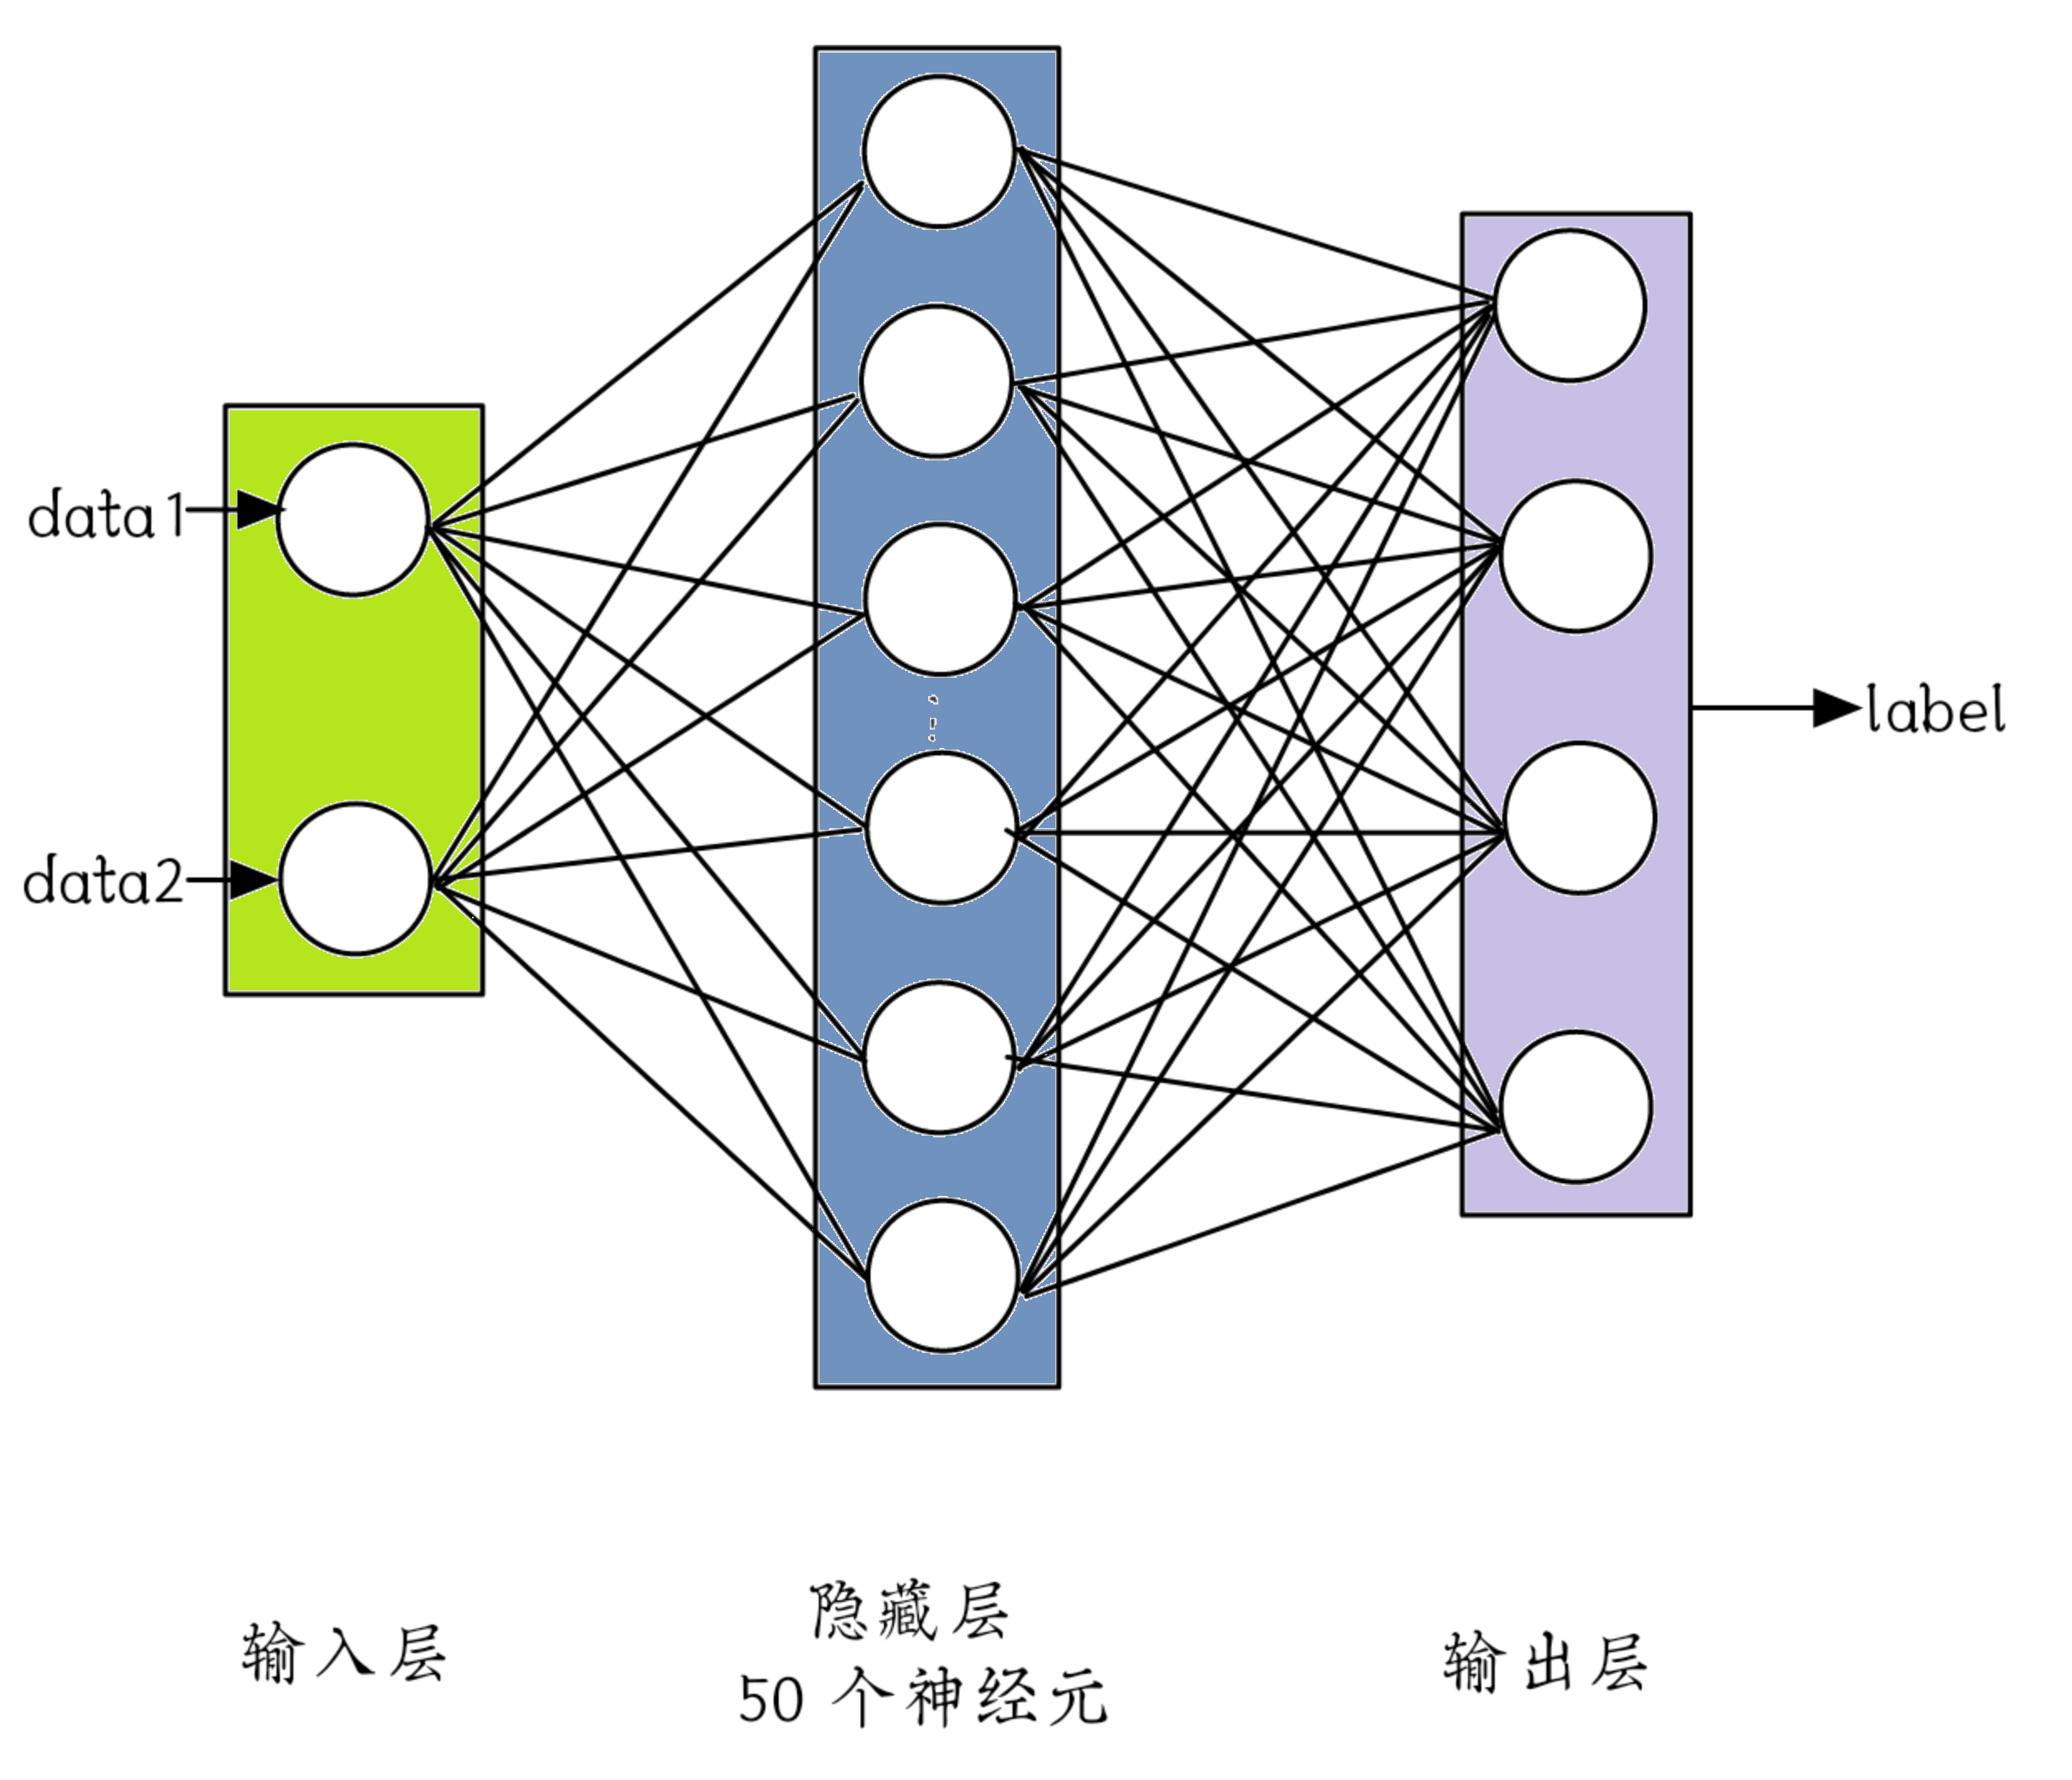
\includegraphics[scale=0.20]{../images/网络架构.png}
		\caption{模型架构图}
		\label{FC模型结构图}
	\end{center}
\end{figure}
为了解决训练时各层参数分布不一致的问题(ICS),使模型更加容易训练,我们在模型的每一个线性层和激活函数层之间
添加了批量正则化(BatchNorm1d)层。另外,为了缓解可能出现的过拟合现象,我们还在每一个激活函数层后添加了 Dropout 层。
经过对超参数的网格搜索寻优,我们将 Dropout 的概率设置为 0.4。
\subsection{损失函数}
损失函数是度量当前分类器的输出和真实值的差异的函数。
本实验要求完成一个 4 分类任务。所以,我们交叉熵损失来作为我们的损失函数。
交叉熵是一种多分类任务中常用的损失函数。假设分类器的输出向量 $p\in R^c$,
真实值的独热向量为 $q\in R^c$。那么交叉熵 $H(p, q)$ 的计算公式如下。
$$
H(p, q)=-\sum_{i=1}^{c}p_i log(q_i)
$$

除此之外,我们还在损失函数中加入了正则化项。在实验中,我们尝试了 L1 正则化和 L2 正则化两种方法,最终选择了 L1 正则化方法。
下面我们将介绍这两种正则化方法。

L1 正则化通过在损失函数中添加参数的 1-范数来对参数进行约束。
通过 L1 正则化,我们可以得到稀疏的模型参数矩阵,从而实现模型简化和特征选择。L1 正则化 $L1$ 的计算公式如下。
$$
L1=\lambda \sum_{i=1}^n |w_i|
$$
其中,$\lambda$ 是用来调节正则化强度的系数,$w$ 是模型参数矩阵。

L2 正则化通过在损失函数中添加参数的 2-范数来对参数进行约束。
通过 L2 正则化,我们使参数的绝对值减小,从而缓解过拟合现象。L2 正则化 $L2$ 的计算公式如下。
$$
L2=\lambda \sum_{i=1}^n w_i^2
$$
其中,$\lambda$ 是用来调节正则化强度的系数,$w$ 是模型参数矩阵。

综上所述,我们的损失函数计算公式如下:
$$
Loss(p, q) = -\sum_{i=1}^{c}p_i log(q_i)+\lambda \sum_{i=1}^n |w_i|
$$

\subsection{优化器}
优化器用来决定下一步模型的参数如何变化。在本实验中,我们选用 AdamW 优化器。
AdamW 优化器是 Adam 优化器的改进版本。它在 Adam 优化器的基础上增加了权值衰减功能。
Adam 优化器同时考虑指数移动平均的一阶动量和二阶动量以指导参数更新。其计算公式如下。
$$
\begin{aligned}
	m_t&=\beta_1m_{t-1}+(1-\beta_1)g_t\\
	v_t&=\beta_2v_{t-1}+(1-\beta_2)diag(g_t^2)\\
	w_{t+1}&=w_{t}-\alpha\frac{m_t}{\sqrt{v_t}+\epsilon}
\end{aligned}
$$

其中,$m_t, v_t$ 是动量相关参数,$\alpha$ 为学习率,$w_t$ 是参数矩阵,$g_t$ 是梯度。
而 Adamw 优化器在 Adam 优化器的基础上加入了权值衰减系数,$w$ 矩阵的更新公式变为。
$$
w_{t+1}=(1-\lambda \alpha)w_{t}-\alpha\frac{m_t}{\sqrt{v_t}+\epsilon}
$$

由于 AdamW 优化器已经进行了学习率自适应,在本次实验中我们向优化器中传入固定值的学习率,而不在设置
学习率更新策略,使其随训练轮数发生变化。

至此,网络架构设计完成。


\section{实验结果}
\subsection{实验环境}
本实验在一个运算服务器上进行,服务器的配置如表\ref{服务器配置}所示。
\begin{table}[H]
	\centering
	\caption{实验环境表}
	  \begin{tabular}{c|c|c}
		\toprule
	  \multirow{3}[0]{*}{硬件} & CPU   & Intel(R) Xeon(R) CPU E5-2686 v4 @ 2.30GHz \\
			& 内存大小    & 251G \\
			& GPU   & NVIDIA GeForce RTX 3070 Ti \\\hline
	  \multirow{3}[0]{*}{软件} & 操作系统  & Ubuntu 20.04.5 LTS \\
			& 深度学习框架 & PyTorch 1.13.1 \\
			& IDE   & Vscode \\\bottomrule
	  \end{tabular}
	\label{服务器配置}
\end{table}
\subsection{超参数设置}
在本次实验中,为了使结果可复现,我们将随机数种子固定为 1024。我们还使用了 GPU 加速训练。
之后,我们对超参数进行了网格搜索寻优。我们在 13824 种参数组合中进行了网格搜索,最优的参数组合如下。

在网络架构方面,我们使用了含有 1 层隐藏层的全连接网络,隐藏层的神经元个数为 50。
激活函数选择 LeakyReLU,负半轴斜率设置为 0.01。

在训练方面,我们训练了 200 个 epoch。由于显存足够,我们采用全数据集训练,batch size 设置为 3600。
学习率设置为 1.0。dropout 概率设置为 0.4,L1 正则化系数设置为 0.001。

对于优化器,我们选择了 AdamW 优化器,$\beta_1$ 参数为 0.9,$\beta_2$ 参数为 0.999。

\subsection{结果}
首先,我们使用上述的超参数对模型进行了训练,在完成每一轮训练后我们将模型在验证集上进行验证。验证所使用的评价指标
包括准确率和 macro f1 分数。我们选择验证集上准确率最高的模型参数进行保存。训练过程中的训练集损失函数值变化和验证集
损失函数值变化如图\ref{训练验证损失函数}所示,验证集上的准确率和 macro f1 分数变化如图\ref{训练验证acc}和\ref{训练验证f1}所示。
\begin{figure}[H]
	\begin{center}
		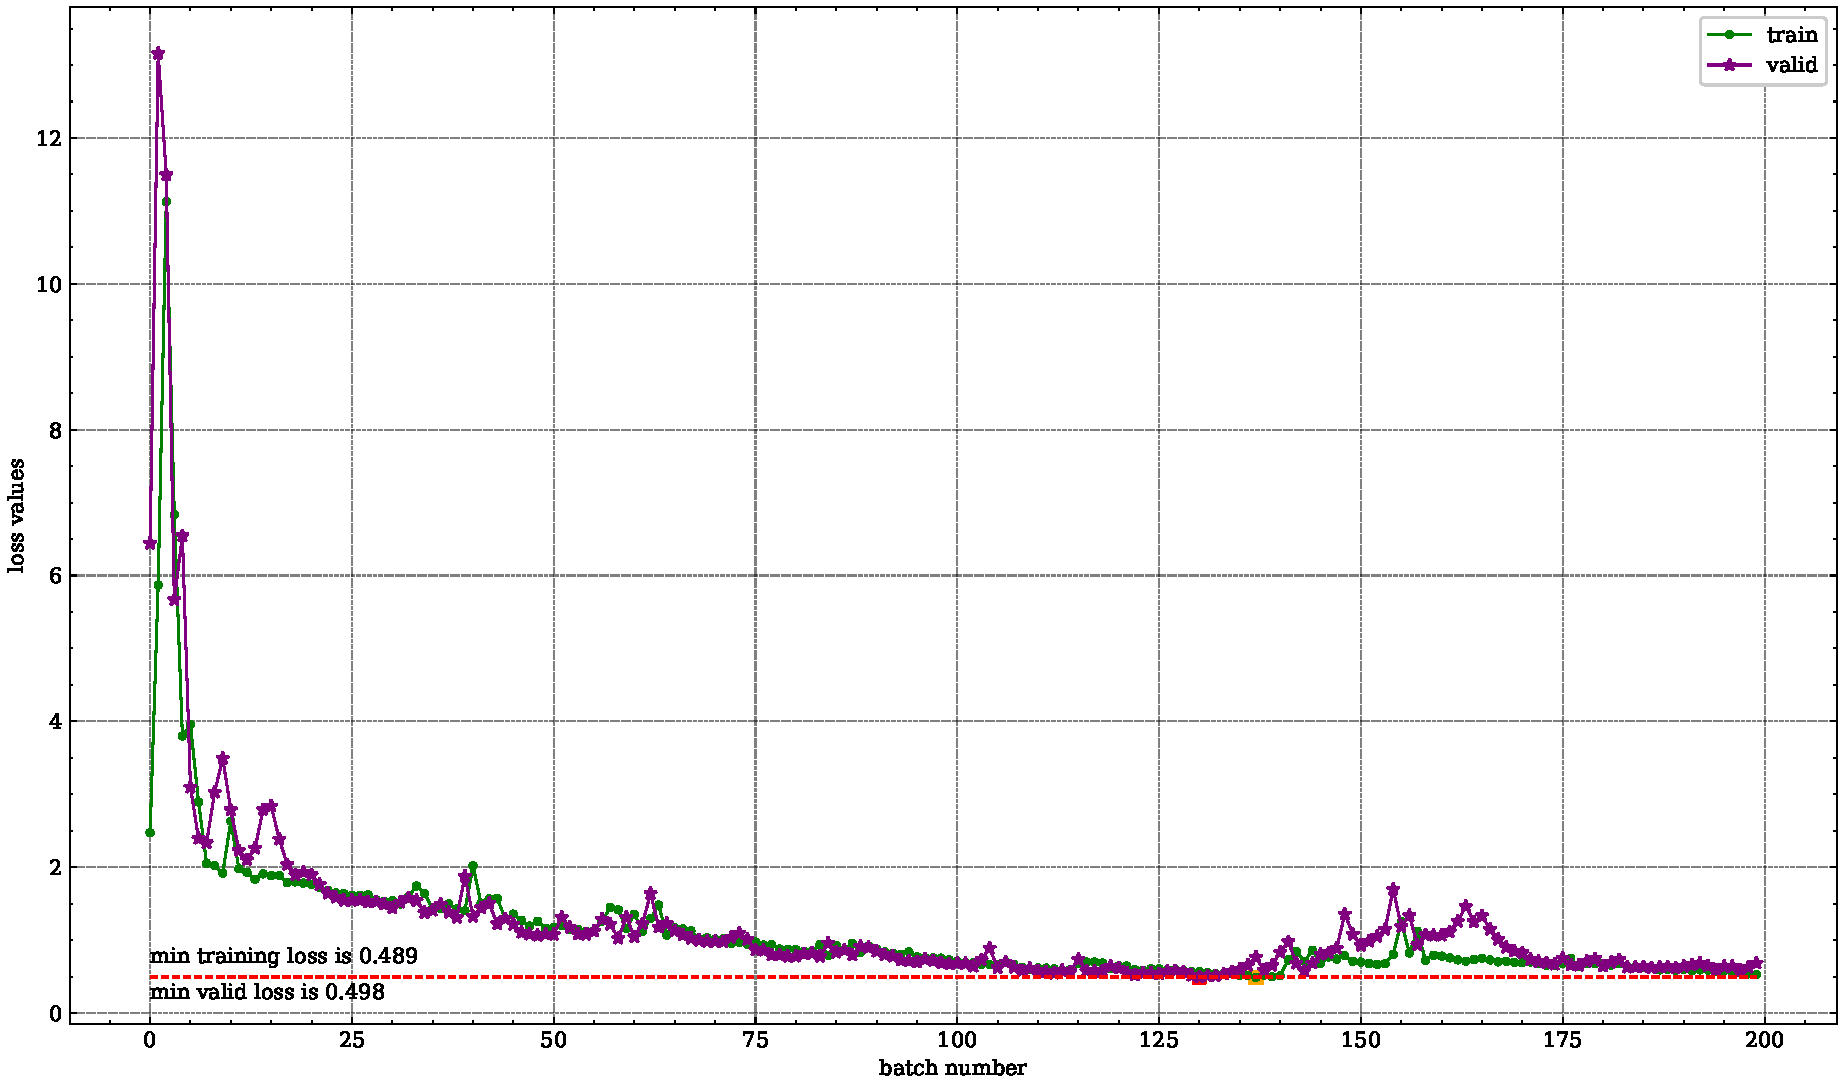
\includegraphics[scale=0.35]{../images/训练验证损失函数.pdf}
		\caption{损失函数变化图}
		\label{训练验证损失函数}
	\end{center}
\end{figure}
\begin{figure}[H]
	\begin{center}
		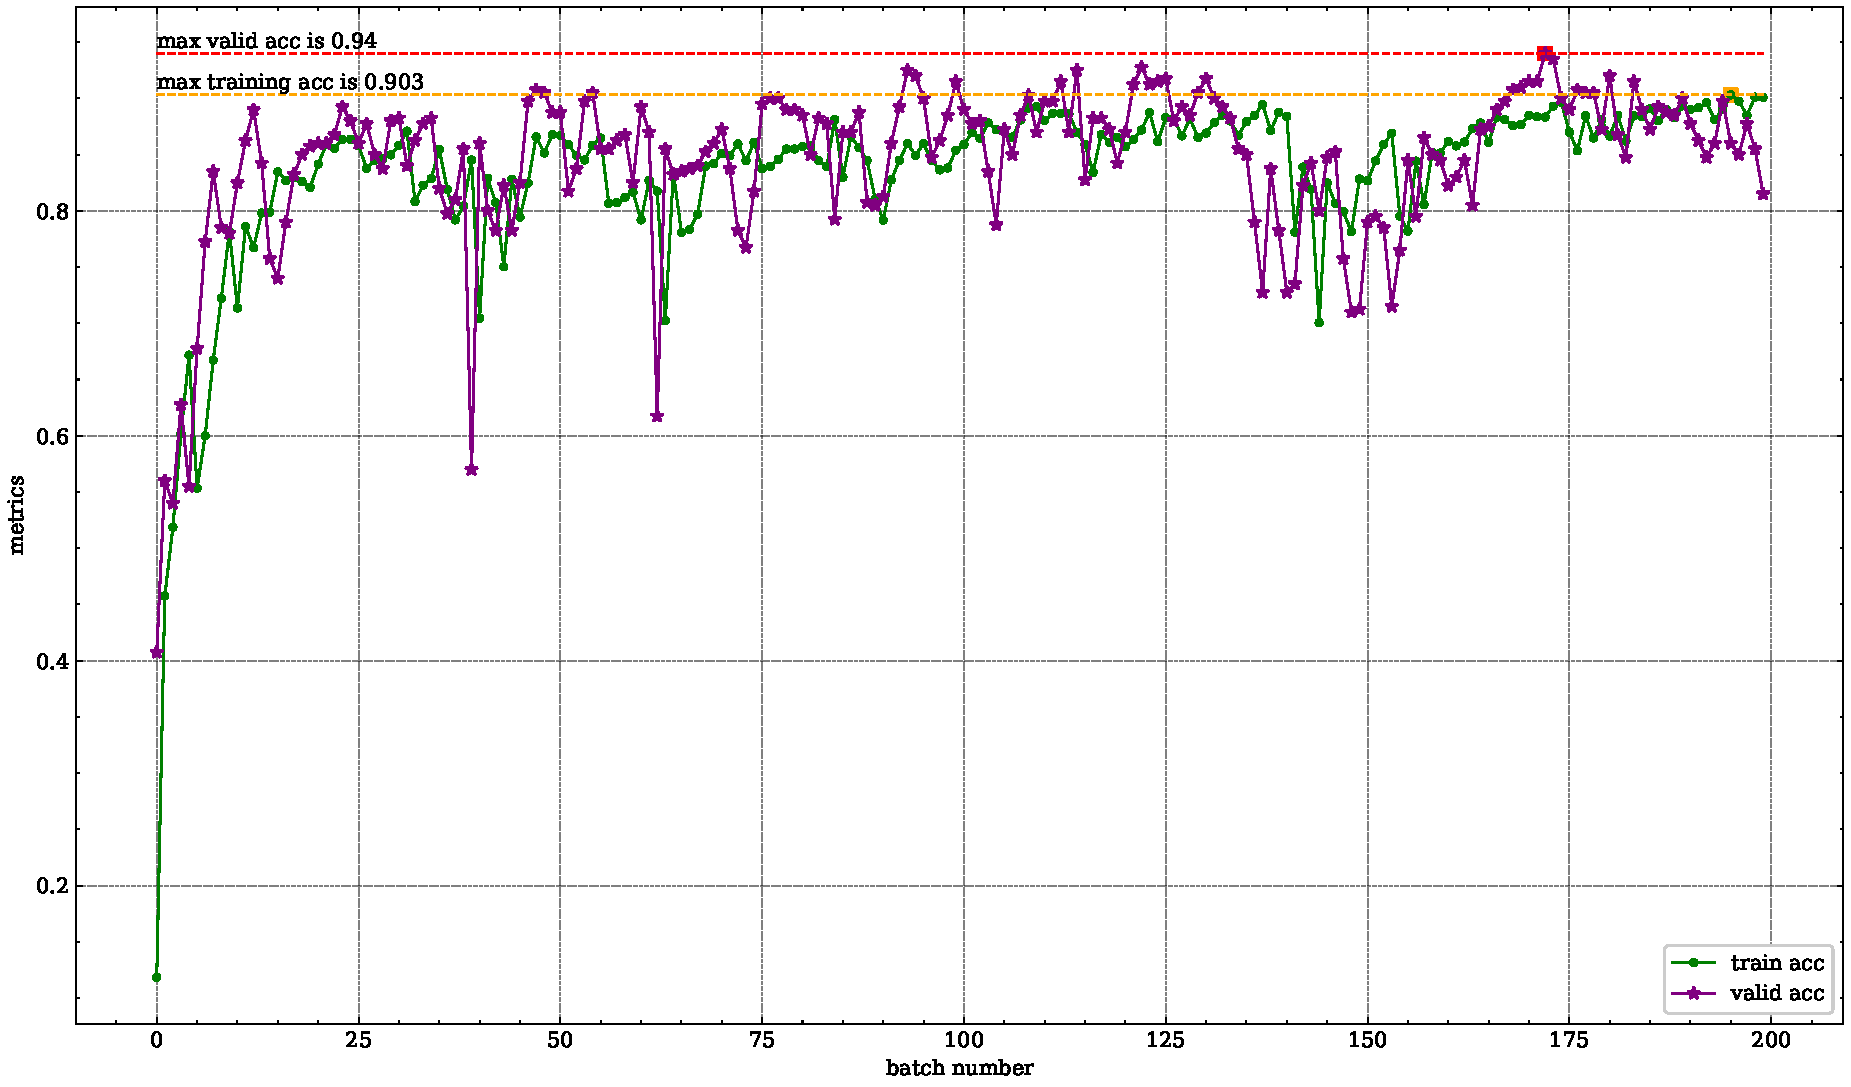
\includegraphics[scale=0.35]{../images/训练验证acc.pdf}
		\caption{准确率变化图}
		\label{训练验证acc}
	\end{center}
\end{figure}
\begin{figure}[H]
	\begin{center}
		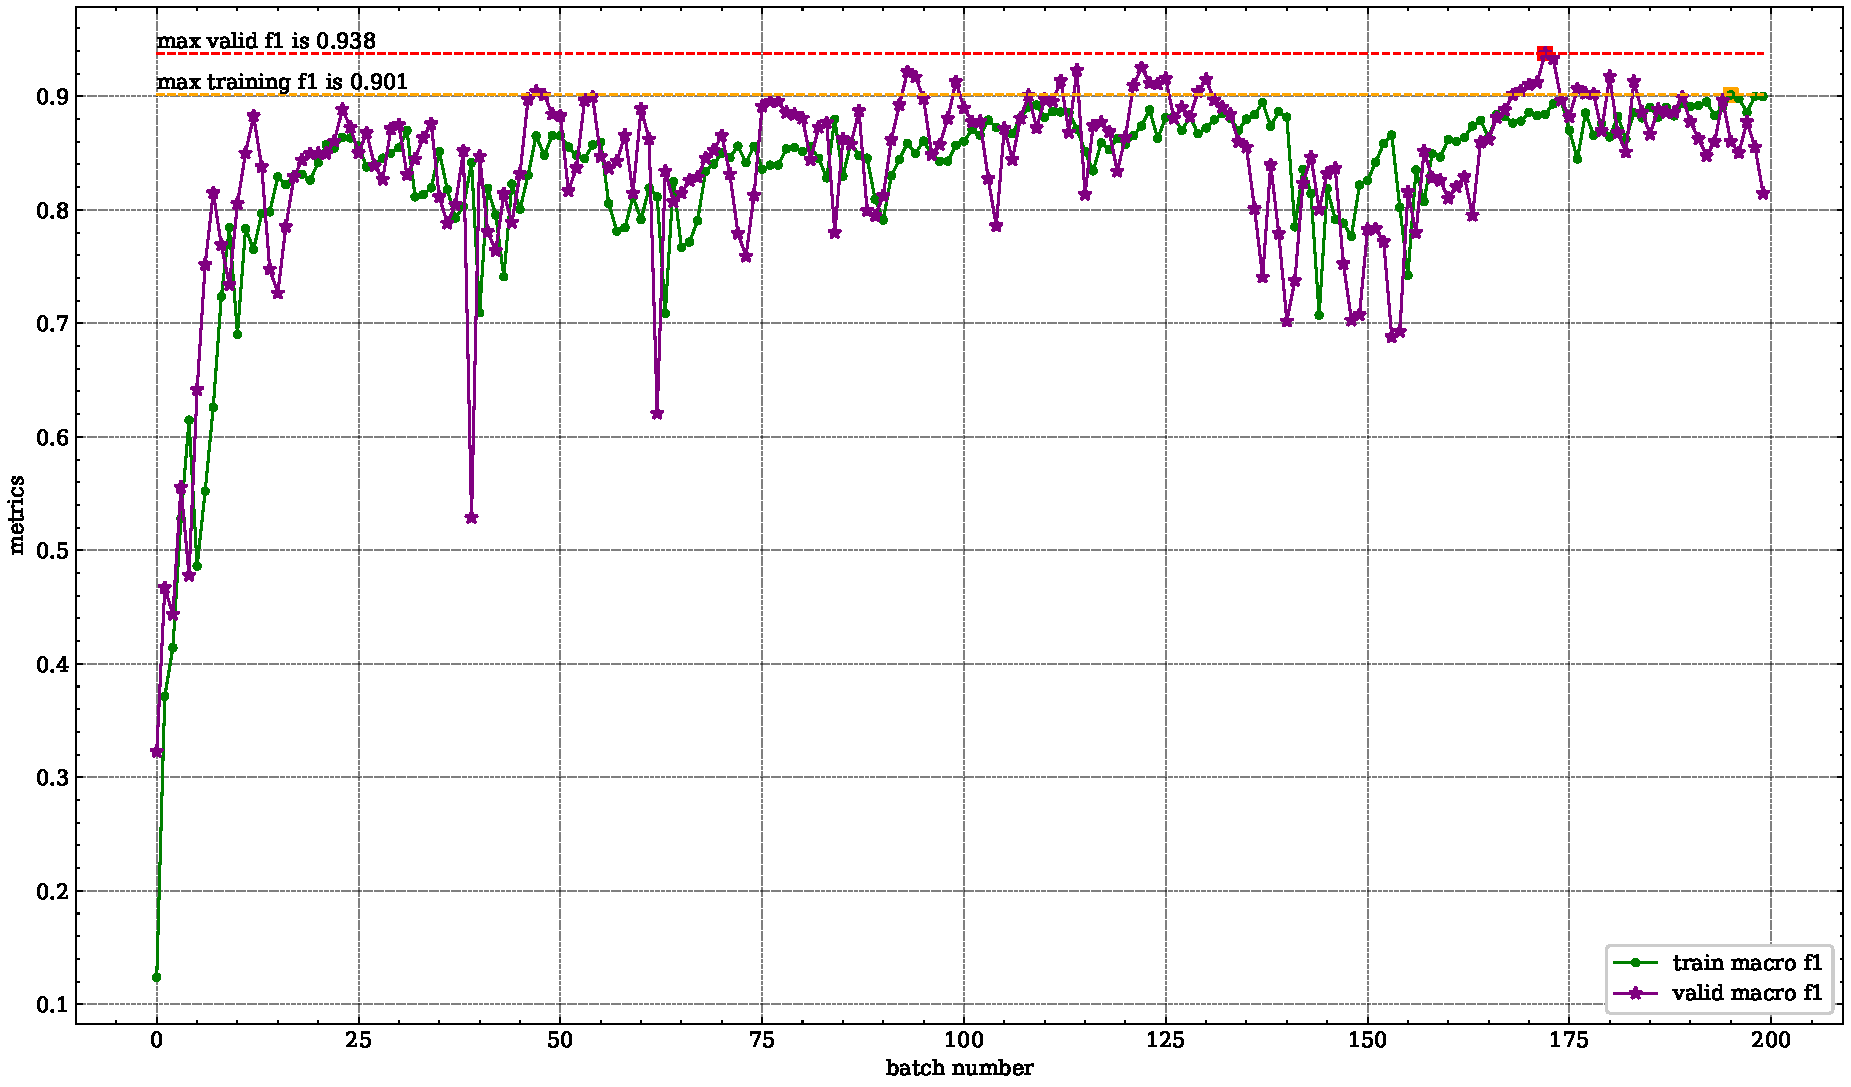
\includegraphics[scale=0.35]{../images/训练验证f1.pdf}
		\caption{macro f1 分数变化图}
		\label{训练验证f1}
	\end{center}
\end{figure}

训练完成后,我们加载保存的最优参数进行测试。在测试中,模型在验证集上的准确率达到了 0.940,marco f1 分数也达到了 0.938。
各类别的相关评价指标如表\ref{各类别评价指标}所示。
\begin{table}[H]
	\centering
	\caption{各类别的相关评价指标}
	  \begin{tabular}{ccccc}
		\toprule
			& \textbf{precision} & \textbf{recall} & \textbf{f1-score} & \textbf{support} \\\hline
	  \textbf{1} & 0.94  & 0.81  & 0.87  & 97 \\
	  \textbf{2} & 0.92  & 0.99  & 0.95  & 105 \\
	  \textbf{3} & 0.96  & 0.97  & 0.97  & 107 \\
	  \textbf{4} & 0.94  & 0.98  & 0.96  & 91 \\
	  \textbf{accuracy} &       &       & 0.94  & 400 \\
	  \textbf{macro avg} & 0.94  & 0.94  & 0.94  & 400 \\
	  \textbf{weighted avg} & 0.94  & 0.94  & 0.94  & 400 \\
	  \bottomrule
	  \end{tabular}
	\label{各类别评价指标}
  \end{table}
  
为了更直观地可视化模型的分类边界,我们绘制了最优模型的分类边界图\ref{模型的分类结果}。
\begin{figure}[H]
	\begin{center}
		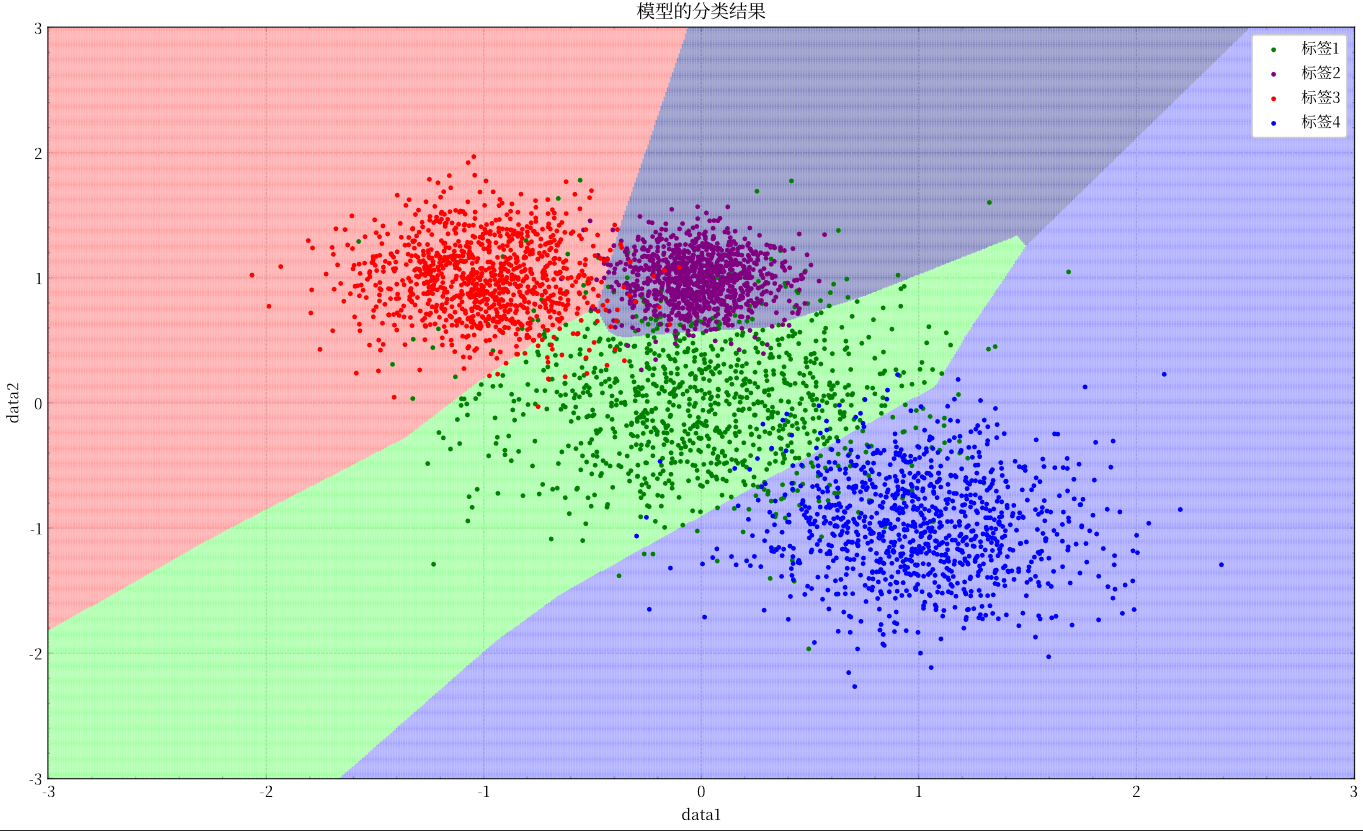
\includegraphics[scale=0.45]{../images/模型的分类结果.pdf}
		\caption{最优模型的分类边界}
		\label{模型的分类结果}
	\end{center}
\end{figure}
图\ref{模型的分类结果}中可见模型基本学习到了 4 个二维高斯分布的大致分类边界,从而获得了较高的准确率和 marco f1 分数。
但由于这 4 个二维高斯分布存在较大的重叠区域,离群值较多,所以模型也无法对所有样本进行正确分类。

\section{总结与讨论}
在这一章,我们研究了不同超参数变化对模型准确率的影响。结果如下。
\subsection{不同的网络层数对准确率的影响}
我们保持除学习率和网络层数外的其它超参数不变,依次将网络层数设置为 1 到 10 层。并调整学习率使得每个网络的效果均达到最优。
接着对每个网络进行训练并测试其准确率。
结果如图\ref{不同的网络层数}所示。
\begin{figure}[H]
	\begin{center}
		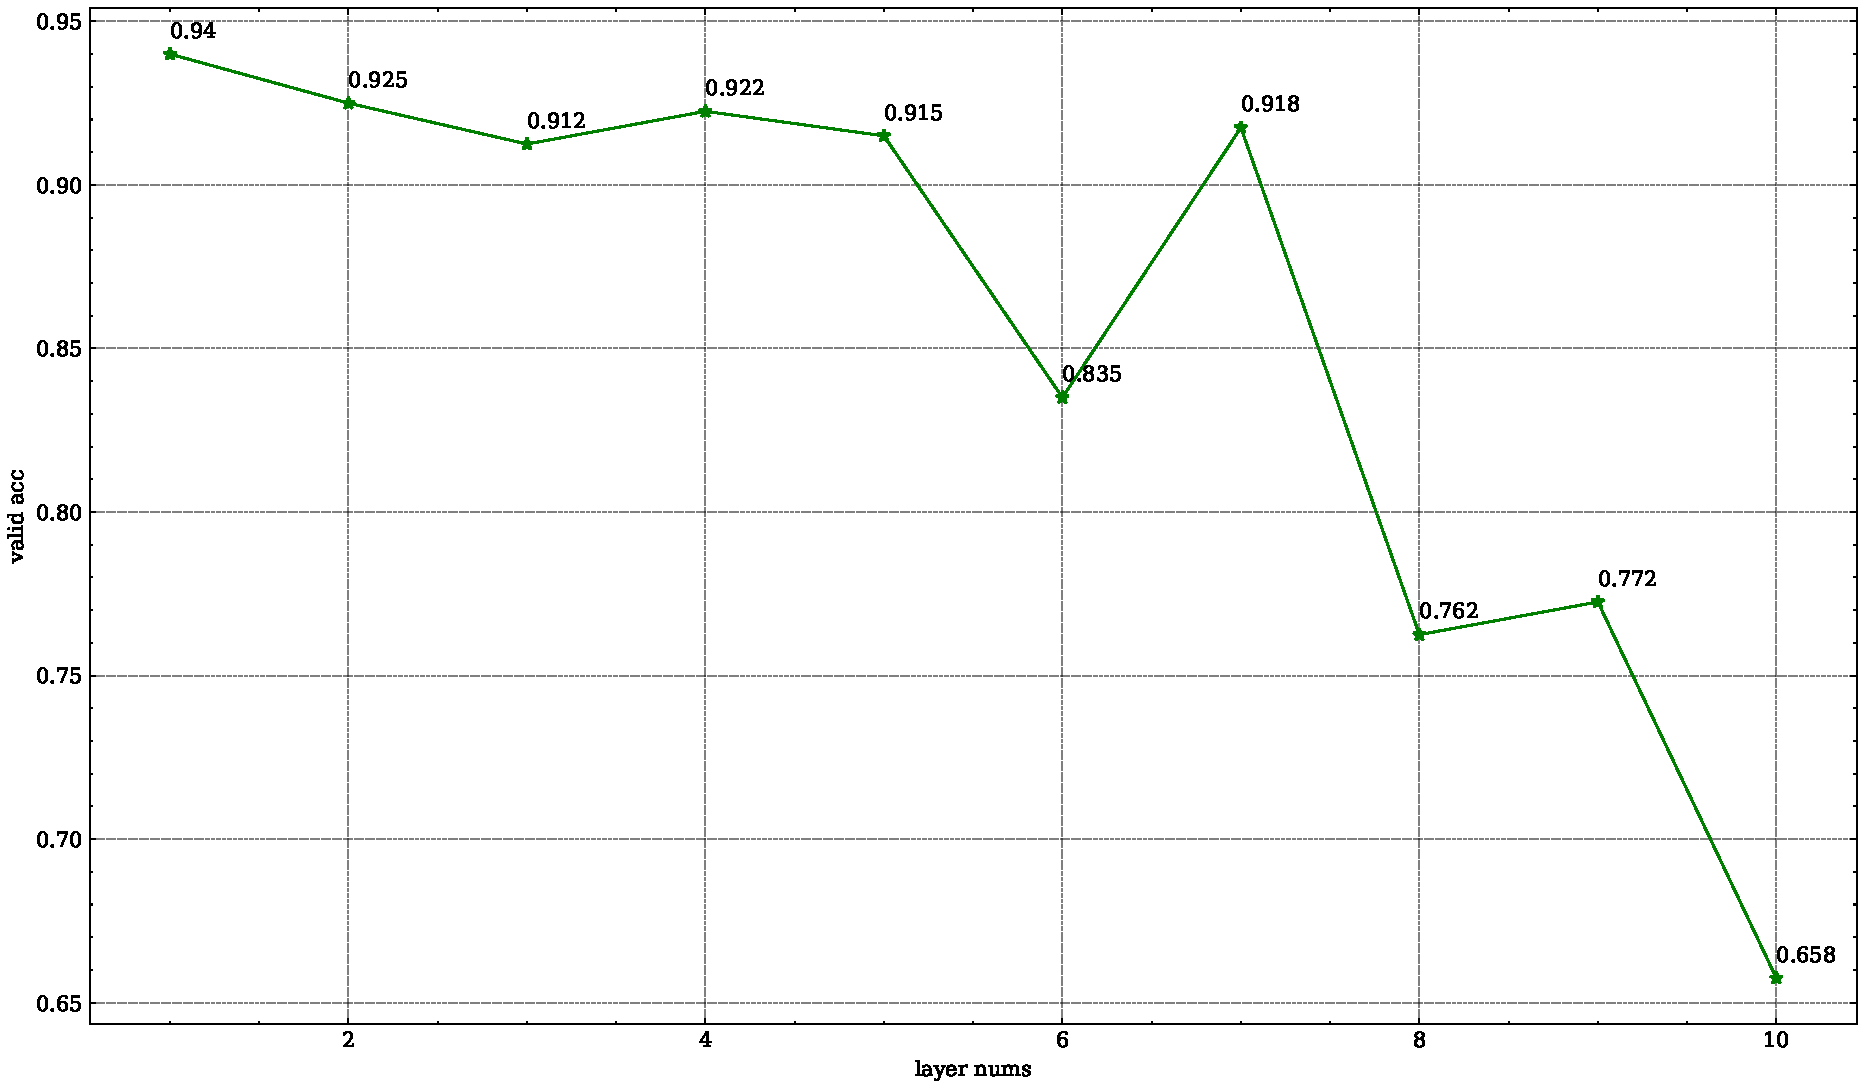
\includegraphics[scale=0.35]{../images/不同的网络层数.pdf}
		\caption{不同的网络层数对准确率的影响}
		\label{不同的网络层数}
	\end{center}
\end{figure}

从图\ref{不同的网络层数}中我们可以看出,随着神经网络层数的增加,模型的效果反而会有所下降,
下降的趋势在层数大于 7 时更为明显。这可能是由于随着神经网络层数的增加,模型的参数量越来越大。
这虽然会使得模型的学习能力提高,但我们的数据集比较小,模型可能无法充分学习有效的特征表示,导致效果下降。
同时,层数较多的模型梯度有较高梯度爆炸或梯度消失的风险,这也会使得效果下降。

综上所述,选择 1 层隐藏层的全连接网络即可得到较好的效果,无需再增加多余的隐藏层。

\subsection{不同的神经元个数对准确率的影响}
我们保持其它超参数不变,依次将隐藏层的神经元个数设置成 10, 20, 30, ..., 100 个。接着对每个网络进行训练并测试其准确率。
结果如图\ref{不同的神经元个数}所示。
\begin{figure}[H]
	\begin{center}
		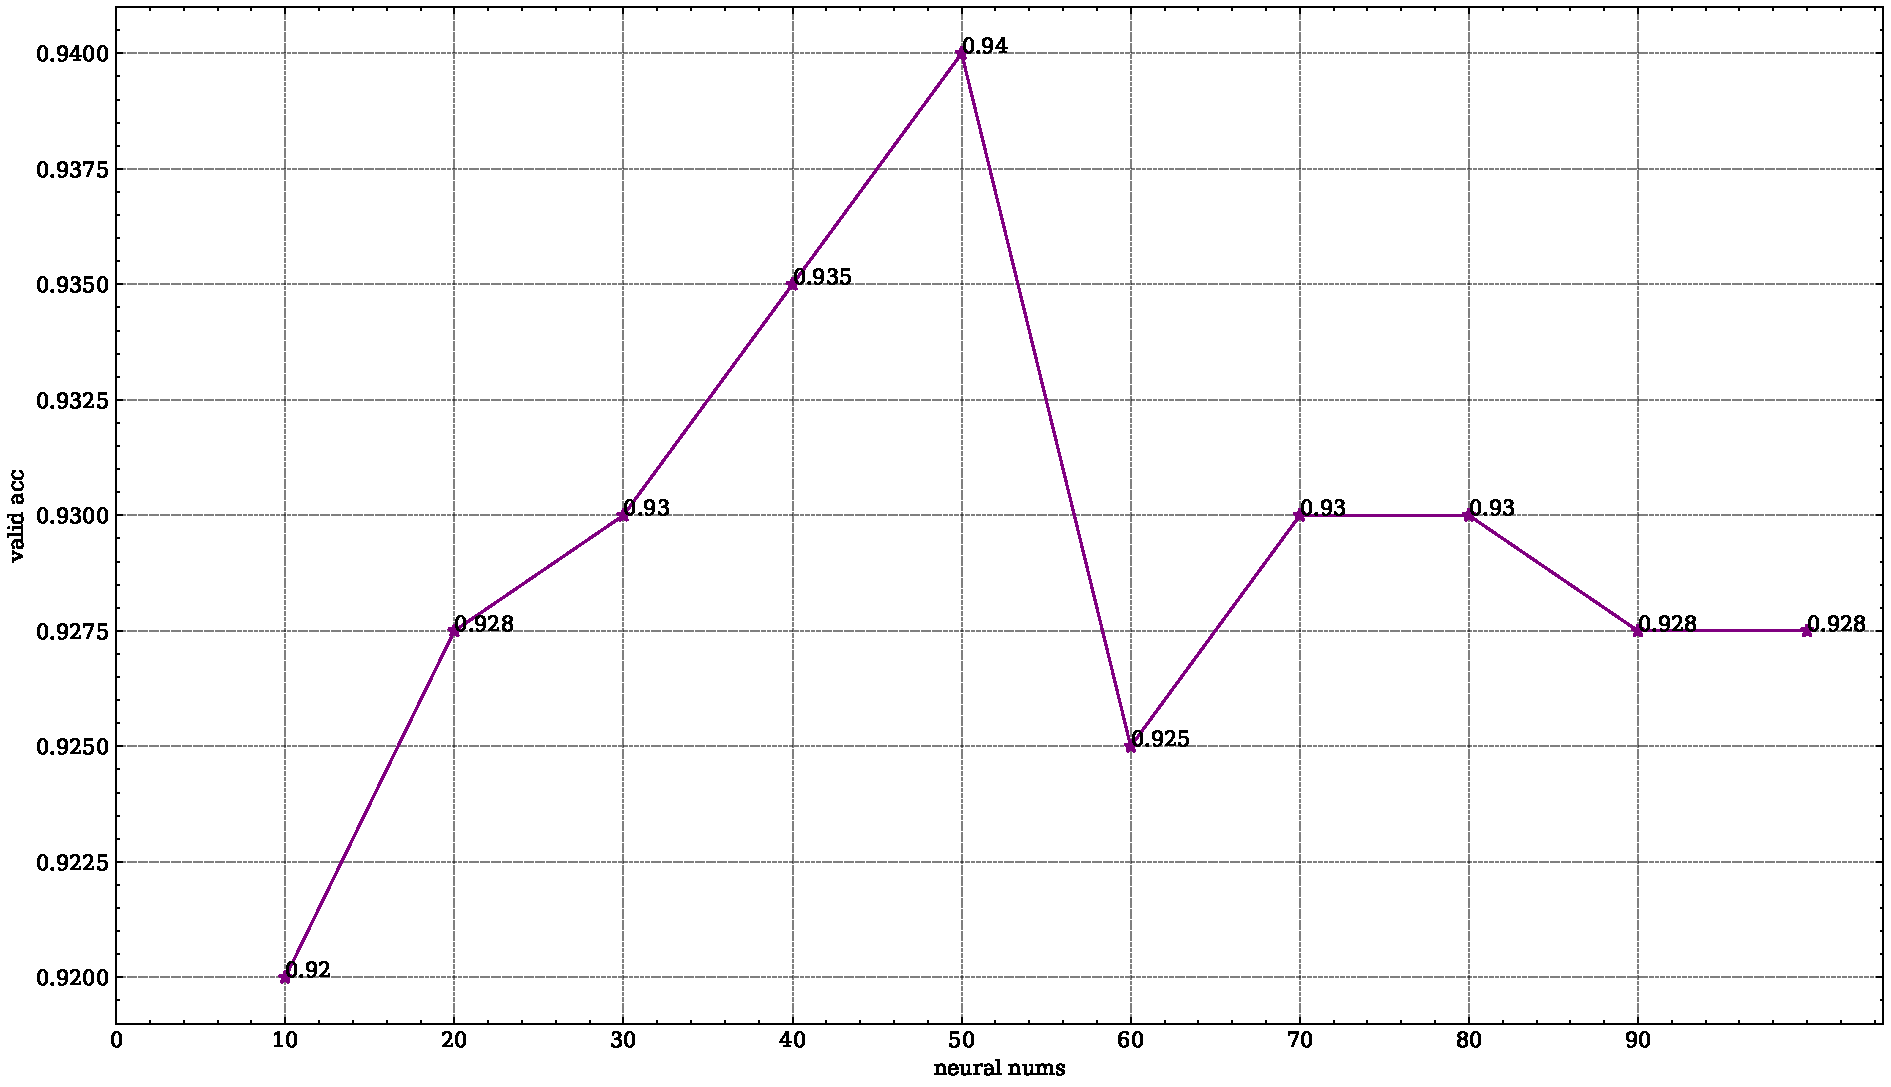
\includegraphics[scale=0.35]{../images/不同的神经元个数.pdf}
		\caption{不同的神经元个数对准确率的影响}
		\label{不同的神经元个数}
	\end{center}
\end{figure}

从图\ref{不同的神经元个数}中我们可以看出,随着隐藏层的神经元个数的增加,
模型的准确率先上升后下降,并在神经元个数为 50 时达到最优值。
这是由于在隐藏层的神经元个数较少时,模型的学习能力不强,无法学到较为深层的特征。
所以随着神经元个数的增加,模型效果越来越好。在隐藏层的神经元个数较多时,受数据集大小的限制,模型可能会发生难以避免的过拟合现象,导致效果下降。
同时过多的隐藏层特征也会导致维度灾难,这加剧了模型的过拟合,故模型效果反而变差。

综上所述,全连接网络隐藏层的神经元个数为 50 时效果最好。

\subsection{不同的学习率对准确率的影响}
我们保持除学习率和最大训练轮数外的其它超参数不变,
依次将学习率设置成 $10^{-6}, 10^{-5}, ..., 1, 10, 50$。
并适当调整最大训练轮数使得使得每个网络的效果均达到最优。
接着对每个网络进行训练并测试其准确率。
结果如图\ref{不同的学习率}所示。
\begin{figure}[H]
	\begin{center}
		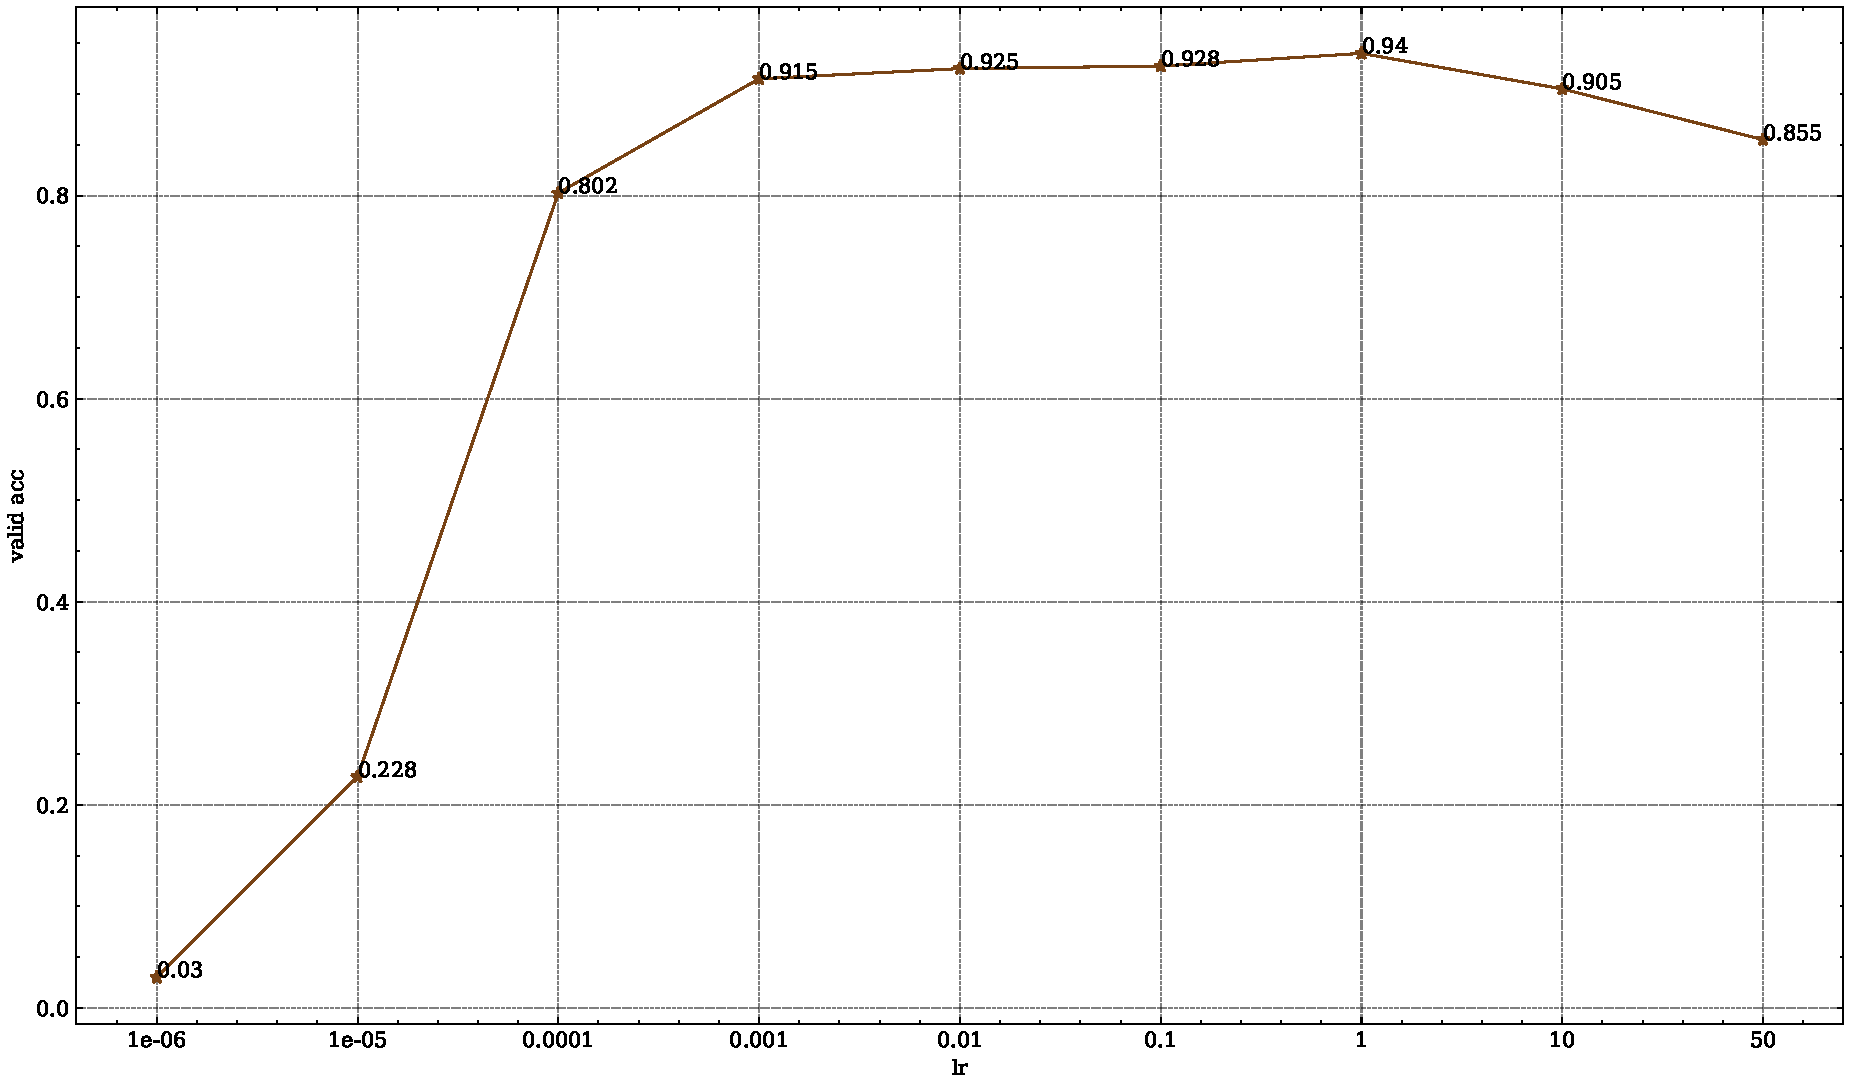
\includegraphics[scale=0.35]{../images/不同的学习率.pdf}
		\caption{不同的学习率对准确率的影响}
		\label{不同的学习率}
	\end{center}
\end{figure}

从图\ref{不同的学习率}中我们可以看出,随着学习率的增加,
模型的准确率先上升后下降,并在学习率为 1 时达到最优值。这是因为当学习率较小时,模型很容易陷入局部极小值。
所以随着学习率的增大,模型效果显著提升。当学习率较大时,模型可能会在极小值附近震荡无法收敛。
所以随着学习率的继续增大,模型效果会下降。

综上所述,学习率设置为 1 时效果最好。
\subsection{不同的 L1 正则化系数对准确率的影响}
我们保持其它超参数不变,依次将 L1 正则化系数设置成 $0, 10^{-4}, 10^{-3}, ..., 1$。接着对每个网络进行训练并测试其准确率。
结果如图\ref{不同的l1_weight}所示。
\begin{figure}[H]
	\begin{center}
		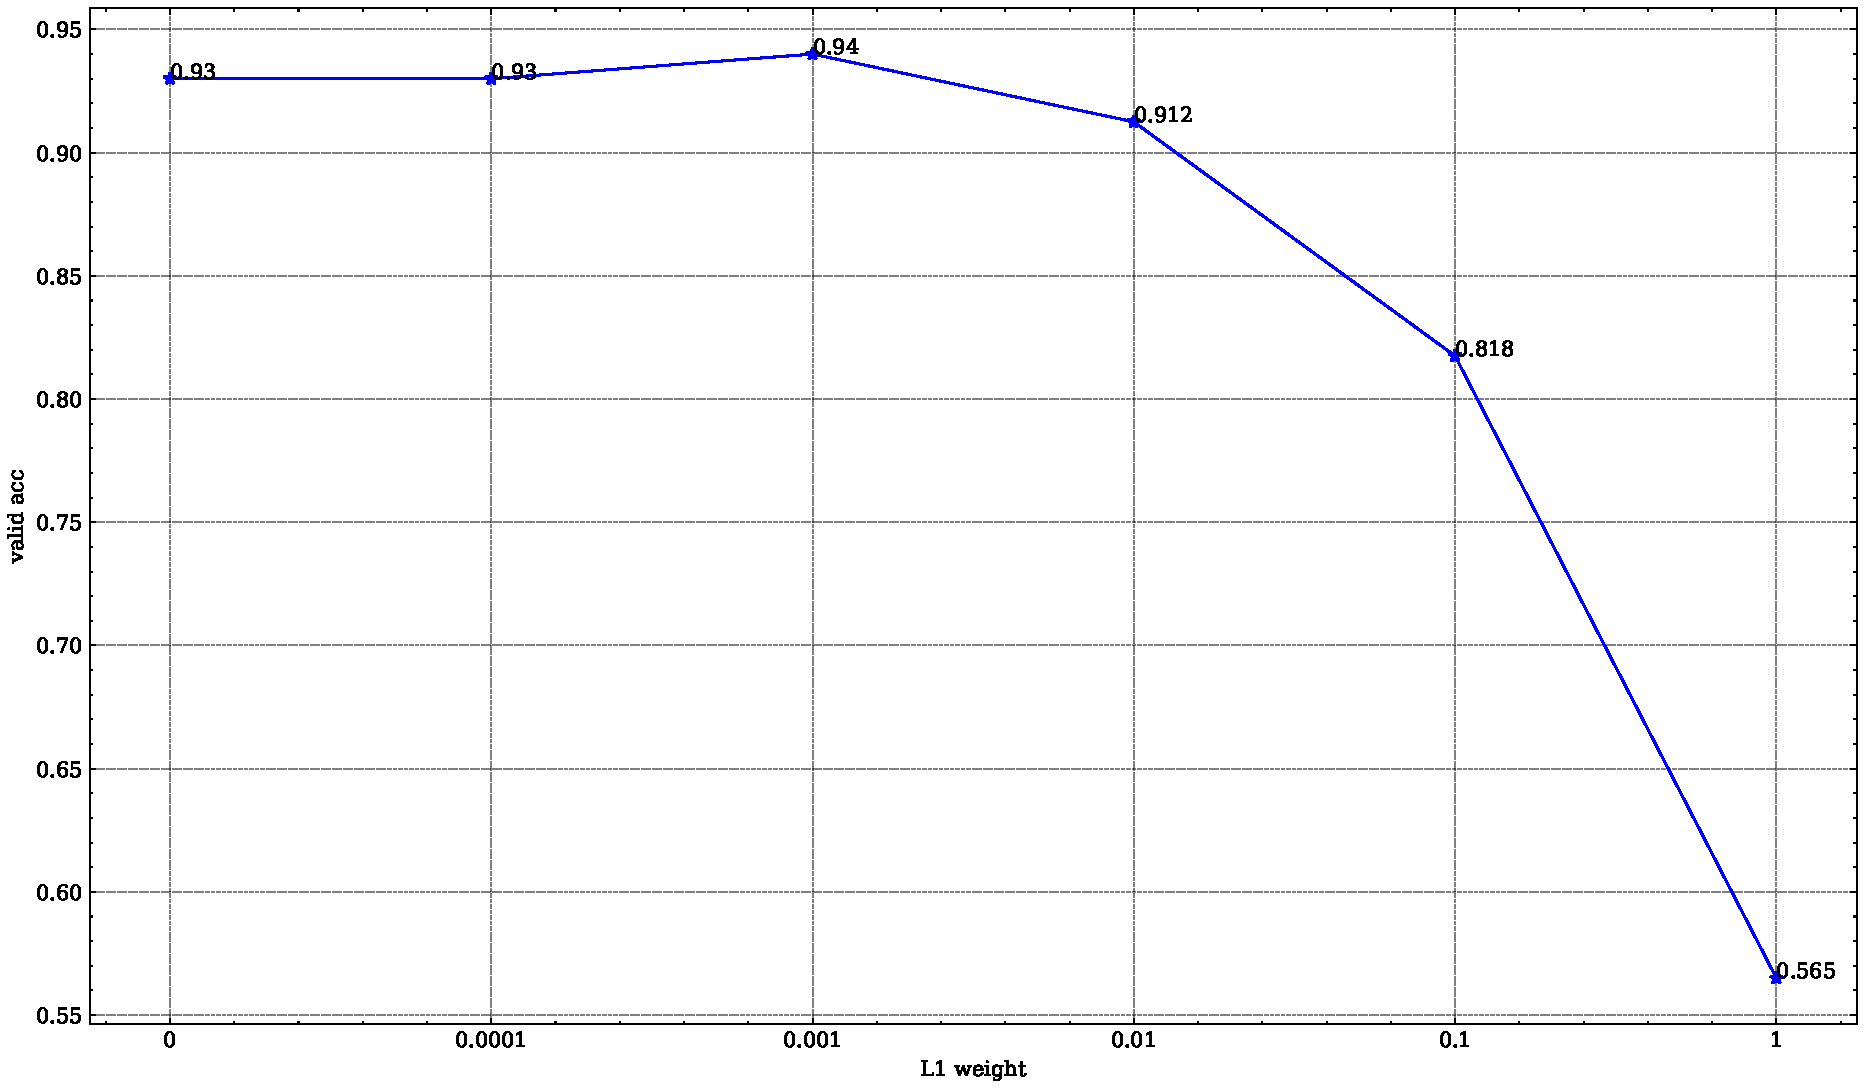
\includegraphics[scale=0.35]{../images/不同的l1_weight.pdf}
		\caption{不同的 $L1$ 正则化系数对准确率的影响}
		\label{不同的l1_weight}
	\end{center}
\end{figure}

从图\ref{不同的l1_weight}中我们可以看出,随着 L1 正则化系数的增加,模型的准确率先略微上升,后迅速下降。
这是由于 L1 正则化可以使得模型的权重稀疏化。当 L1 正则化系数较小时,模型会保留更多的特征,这其中可能有对模型预测有负面影响的无用特征。
所以,当 L1 正则化系数增加时,模型的准确率会略微上升。
如果 L1 正则化系数过大,模型的权重会被过度稀疏化,导致模型过于简单,无法充分学习训练数据,发生欠拟合。
同时,模型还会舍弃一些有用特征。所以,当 L1 正则化系数继续增加时,模型的准确率会迅速下降。

综上所述,模型的 L1 正则化系数设置成 0.001 时效果最好。

\subsection{不同的激活函数对准确率的影响}
我们保持其它超参数不变,依次将激活函数设置成 LeakyReLU, ReLU, Sigmoid, GELU。接着对每个网络进行训练并测试其准确率。
结果如表\ref{不同的激活函数}所示。
\begin{table}[H]
	\centering
	\caption{不同的激活函数对准确率的影响}
	  \begin{tabular}{c|cccc}
		\toprule
	  \textbf{激活函数} & Sigmoid & ReLU  & LeakyReLU & GELU \\\hline
	  \textbf{准确率} & 0.935 & 0.928 & 0.94  & 0.93 \\
	  \bottomrule
	  \end{tabular}
	\label{不同的激活函数}
  \end{table}

从表\ref{不同的激活函数}中我们可以看出,使用不同激活函数的模型准确率几乎相同。这主要是由于分类任务和我们使用
的模型架构都较为简单,没有梯度爆炸或梯度消失的问题。

\section{实验代码简述}
在本章中,我们简要介绍实验代码的构成。更具体的介绍请见 ReadMe.md 文件。

工作目录中存在 7 个文件和 2 个目录。整个工作目录的结构如下。
\begin{figure}[H]
	\begin{center}
		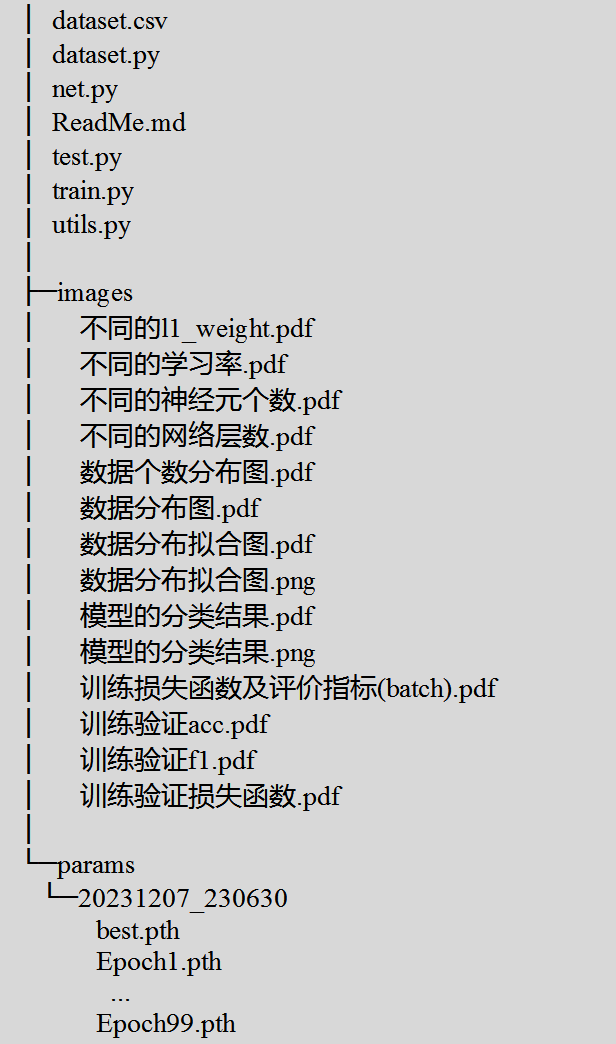
\includegraphics[scale=0.5]{../images/tree.png}
		\caption{工作目录的结构}
	\end{center}
\end{figure}

其中,dataset.csv 是原始数据集。dataset.py 中含有数据预处理的相关函数。net.py 含有模型架构的定义。
ReadMe.md 中介绍了如何对模型进行训练和测试。test.py 是进行模型测试的源代码文件。train.py是进行模型训练的源代码文件。
utils.py 中含有一些工具函数。各函数和类的源代码均含有详细的注释,方便使用者了解其完成的工作。

images 目录存放所有绘制的图像。params 目录存放模型的参数。当在源代码中设置存储参数选项为 True 并运行一次 train.py 时,
params 目录中会增加一个以当前时间为名称的子目录。子目录内存放着每一轮训练结束后的模型参数以及效果最佳的模型参数。

\end{document}